% Options for packages loaded elsewhere
\PassOptionsToPackage{unicode}{hyperref}
\PassOptionsToPackage{hyphens}{url}
%
\documentclass[
  11pt,
]{book}
\usepackage{lmodern}
\usepackage{setspace}
\usepackage{amssymb,amsmath}
\usepackage{ifxetex,ifluatex}
\ifnum 0\ifxetex 1\fi\ifluatex 1\fi=0 % if pdftex
  \usepackage[T1]{fontenc}
  \usepackage[utf8]{inputenc}
  \usepackage{textcomp} % provide euro and other symbols
\else % if luatex or xetex
  \usepackage{unicode-math}
  \defaultfontfeatures{Scale=MatchLowercase}
  \defaultfontfeatures[\rmfamily]{Ligatures=TeX,Scale=1}
\fi
% Use upquote if available, for straight quotes in verbatim environments
\IfFileExists{upquote.sty}{\usepackage{upquote}}{}
\IfFileExists{microtype.sty}{% use microtype if available
  \usepackage[]{microtype}
  \UseMicrotypeSet[protrusion]{basicmath} % disable protrusion for tt fonts
}{}
\makeatletter
\@ifundefined{KOMAClassName}{% if non-KOMA class
  \IfFileExists{parskip.sty}{%
    \usepackage{parskip}
  }{% else
    \setlength{\parindent}{0pt}
    \setlength{\parskip}{6pt plus 2pt minus 1pt}}
}{% if KOMA class
  \KOMAoptions{parskip=half}}
\makeatother
\usepackage{xcolor}
\IfFileExists{xurl.sty}{\usepackage{xurl}}{} % add URL line breaks if available
\IfFileExists{bookmark.sty}{\usepackage{bookmark}}{\usepackage{hyperref}}
\hypersetup{
  pdftitle={Selected Topics In Data Science},
  pdfauthor={Bruce Campbell},
  hidelinks,
  pdfcreator={LaTeX via pandoc}}
\urlstyle{same} % disable monospaced font for URLs
\usepackage{color}
\usepackage{fancyvrb}
\newcommand{\VerbBar}{|}
\newcommand{\VERB}{\Verb[commandchars=\\\{\}]}
\DefineVerbatimEnvironment{Highlighting}{Verbatim}{commandchars=\\\{\}}
% Add ',fontsize=\small' for more characters per line
\usepackage{framed}
\definecolor{shadecolor}{RGB}{248,248,248}
\newenvironment{Shaded}{\begin{snugshade}}{\end{snugshade}}
\newcommand{\AlertTok}[1]{\textcolor[rgb]{0.94,0.16,0.16}{#1}}
\newcommand{\AnnotationTok}[1]{\textcolor[rgb]{0.56,0.35,0.01}{\textbf{\textit{#1}}}}
\newcommand{\AttributeTok}[1]{\textcolor[rgb]{0.77,0.63,0.00}{#1}}
\newcommand{\BaseNTok}[1]{\textcolor[rgb]{0.00,0.00,0.81}{#1}}
\newcommand{\BuiltInTok}[1]{#1}
\newcommand{\CharTok}[1]{\textcolor[rgb]{0.31,0.60,0.02}{#1}}
\newcommand{\CommentTok}[1]{\textcolor[rgb]{0.56,0.35,0.01}{\textit{#1}}}
\newcommand{\CommentVarTok}[1]{\textcolor[rgb]{0.56,0.35,0.01}{\textbf{\textit{#1}}}}
\newcommand{\ConstantTok}[1]{\textcolor[rgb]{0.00,0.00,0.00}{#1}}
\newcommand{\ControlFlowTok}[1]{\textcolor[rgb]{0.13,0.29,0.53}{\textbf{#1}}}
\newcommand{\DataTypeTok}[1]{\textcolor[rgb]{0.13,0.29,0.53}{#1}}
\newcommand{\DecValTok}[1]{\textcolor[rgb]{0.00,0.00,0.81}{#1}}
\newcommand{\DocumentationTok}[1]{\textcolor[rgb]{0.56,0.35,0.01}{\textbf{\textit{#1}}}}
\newcommand{\ErrorTok}[1]{\textcolor[rgb]{0.64,0.00,0.00}{\textbf{#1}}}
\newcommand{\ExtensionTok}[1]{#1}
\newcommand{\FloatTok}[1]{\textcolor[rgb]{0.00,0.00,0.81}{#1}}
\newcommand{\FunctionTok}[1]{\textcolor[rgb]{0.00,0.00,0.00}{#1}}
\newcommand{\ImportTok}[1]{#1}
\newcommand{\InformationTok}[1]{\textcolor[rgb]{0.56,0.35,0.01}{\textbf{\textit{#1}}}}
\newcommand{\KeywordTok}[1]{\textcolor[rgb]{0.13,0.29,0.53}{\textbf{#1}}}
\newcommand{\NormalTok}[1]{#1}
\newcommand{\OperatorTok}[1]{\textcolor[rgb]{0.81,0.36,0.00}{\textbf{#1}}}
\newcommand{\OtherTok}[1]{\textcolor[rgb]{0.56,0.35,0.01}{#1}}
\newcommand{\PreprocessorTok}[1]{\textcolor[rgb]{0.56,0.35,0.01}{\textit{#1}}}
\newcommand{\RegionMarkerTok}[1]{#1}
\newcommand{\SpecialCharTok}[1]{\textcolor[rgb]{0.00,0.00,0.00}{#1}}
\newcommand{\SpecialStringTok}[1]{\textcolor[rgb]{0.31,0.60,0.02}{#1}}
\newcommand{\StringTok}[1]{\textcolor[rgb]{0.31,0.60,0.02}{#1}}
\newcommand{\VariableTok}[1]{\textcolor[rgb]{0.00,0.00,0.00}{#1}}
\newcommand{\VerbatimStringTok}[1]{\textcolor[rgb]{0.31,0.60,0.02}{#1}}
\newcommand{\WarningTok}[1]{\textcolor[rgb]{0.56,0.35,0.01}{\textbf{\textit{#1}}}}
\usepackage{longtable,booktabs}
% Correct order of tables after \paragraph or \subparagraph
\usepackage{etoolbox}
\makeatletter
\patchcmd\longtable{\par}{\if@noskipsec\mbox{}\fi\par}{}{}
\makeatother
% Allow footnotes in longtable head/foot
\IfFileExists{footnotehyper.sty}{\usepackage{footnotehyper}}{\usepackage{footnote}}
\makesavenoteenv{longtable}
\usepackage{graphicx,grffile}
\makeatletter
\def\maxwidth{\ifdim\Gin@nat@width>\linewidth\linewidth\else\Gin@nat@width\fi}
\def\maxheight{\ifdim\Gin@nat@height>\textheight\textheight\else\Gin@nat@height\fi}
\makeatother
% Scale images if necessary, so that they will not overflow the page
% margins by default, and it is still possible to overwrite the defaults
% using explicit options in \includegraphics[width, height, ...]{}
\setkeys{Gin}{width=\maxwidth,height=\maxheight,keepaspectratio}
% Set default figure placement to htbp
\makeatletter
\def\fps@figure{htbp}
\makeatother
\setlength{\emergencystretch}{3em} % prevent overfull lines
\providecommand{\tightlist}{%
  \setlength{\itemsep}{0pt}\setlength{\parskip}{0pt}}
\setcounter{secnumdepth}{5}
\usepackage{booktabs}

This work is a collection of data science, machine learning, and statistics notes taken in the last few years. No effort has been made to be complete with citations, references, or attribution.  This is merely the results of lots of google queries and trials with various algorithms, software packages, and methods.
\usepackage[]{natbib}
\bibliographystyle{plainnat}

\title{Selected Topics In Data Science}
\author{Bruce Campbell}
\date{2021-08-26}

\begin{document}
\maketitle

\setstretch{1.2}
\hypertarget{preface}{%
\chapter{Preface}\label{preface}}

This is the first installment on my promise to elucidate less popular topics in statistics and machine learning. I wrote this as a way to solidify my understanding of some of the topics that are treated here. Hopefully others will find value here.

\hypertarget{intro}{%
\chapter{Introduction}\label{intro}}

``Where must we go, we who wander this wasteland, in search of our better selves.'' -The First History of Man

This is a living book. It's under development. We are using the \textbf{bookdown} package \citep{R-bookdown} in this book, which was built on top of R Markdown and \textbf{knitr} \citep{xie2015}.

\hypertarget{data-science-best-practices-and-processes}{%
\chapter{Data Science Best Practices and Processes}\label{data-science-best-practices-and-processes}}

This (draft) document is meant to help onboard new data scientists and serve as a reference for current data scientists. Data science consists of a multidisciplinary field encompassing machine learning \& statistics, knowledge representation, visualization, writing, and software engineering. This document covers a variety of subjects and best practices from how to run an Agile data science process, to coding standards, and to project management.

There is no right way to do data science but many ways to do it wrong. This document represents just one approach. Data science is a team sport, and consensus is the best way to define what process works best.

Above all else, we're scientists, and that comes with ethical and process implications. Keep this in mind always.

\hypertarget{code-of-conduct}{%
\section{Code of Conduct}\label{code-of-conduct}}

We don't have a strict code of conduct here, but there are a few essential principles we hold dear:

\begin{itemize}
\tightlist
\item
  Act in good faith: we are here to accomplish several goals - deliver value to the company, one another, and ourselves. Whenever you have a choice to make about work or how you treat a colleague, ask whether, in doing so, you further these goals.
\item
  Consider things from other people's perspectives: Working on a team is hard if we expect our colleagues to do all the work of communication. Give people the benefit of the doubt when you disagree, and try to understand what they are really saying and why they might be doing so.
\item
  Create a welcoming environment: This team recognizes that racism, sexism, gender discrimination, and classism can severely impact the way people move through both life and the workplace. It is our policy to proactively address these problems by educating ourselves about them, self-monitoring and letting our colleagues, regardless of their background, get on with work. At the same time, we actively seek to improve the work environment.
\end{itemize}

\hypertarget{ethics}{%
\section{Ethics}\label{ethics}}

Ethics is an essential concern in machine learning. Focusing on the ethical impact of a model will potentially reduce bias and improve results. Try to think through the hidden biases and potential misuses of any model you build. Think about this in model choice - try to use transparent methods like traditional statistical models and decision trees when interpretability is important.

8 Principles for ethical machine learning.
{[}\url{https://ethical.institute/}{]}

\begin{itemize}
\item
  Human augmentation: assess the impact of incorrect predictions and, when reasonable, design systems with human-in-the-loop review processes.
\item
  Bias evaluation: continuously develop processes that allow me to understand, document, and monitor bias in development and production.
\item
  Explainability by justification: develop tools and processes to continuously improve transparency and explainability of machine learning systems where reasonable.
\item
  Reproducible operations: develop the infrastructure required to enable for a reasonable level of reproducibility across the operations of ML systems.
\item
  Displacement strategy: identify and document relevant information so that business change processes can be developed to mitigate the impact towards workers being automated.
\item
  Practical accuracy: develop processes to ensure my accuracy and cost metric functions are aligned to the domain-specific applications.
\item
  Trust by privacy: build and communicate processes that protect and handle data with stakeholders that may interact with the system directly and/or indirectly.
\item
  Data risk awareness: develop and improve reasonable processes and infrastructure to ensure data and model security are being taken into consideration during the development of machine learning systems.
\end{itemize}

\hypertarget{project-philosophy}{%
\chapter{Project Philosophy}\label{project-philosophy}}

Projects should, to the best of our ability, be broken up into as many small pieces as possible and is feasible. Dependencies between projects should be managed by tools and proper software configuration management (packages) rather than by including code from one project directly inside another project.

This practice encourages modular design and also encourages independence between projects. Sometimes it is better to implement multiple similar pieces of code in different projects than it is to expect a single library to cover all of these slightly different cases in a simple, coherent way.

When a subset of a project reaches the point of being its own library or utility, don't be afraid to factor it out - git can even preserve the history of the sub-project in a new repository for you.

Many choices we make as software developers are arbitrary, in the sense that they don't significantly impact productivity. Whether a team uses R or Python is probably one such choice, for instance, since both languages provide roughly the same capabilities or their costs and benefits balance out. The value of fixing such decisions isn't in the choices themselves, but on reducing the complexity of the development process for the data science community at large. In other words, while we strive to find the best possible practices to use, don't take this document as bald assertions that these are the optimal choices. The point is to simplify teamwork, collaboration, and add clarity to our process.

\hypertarget{project-planning-and-accounting}{%
\chapter{Project Planning and Accounting}\label{project-planning-and-accounting}}

Data science should be run in an Agile fashion. Agile is a general type of project management process, used mainly for software development, where and solutions evolve through the collaborative effort of self-organizing. This includes Kanban and SCRUM.

\begin{itemize}
\tightlist
\item
  Generally, a data scientist will work on only one or two projects per sprint.
\item
  Project artifacts should be stored in content stores like Rally/Jira, Confluence/Mojo
\item
  Code, documentation and all software artifacts for a project \emph{must} exist in a git repository
\item
  Data and private information should \emph{not} exist in any git repository. Automation in each project should, instead, fetch necessary data to a location outside the git repository (or ignored by it). Instructions about where to get private information required for the project should be in the project documentation.
\item
  Projects must have defined completion criteria before starting
\end{itemize}

Project planning is hard. The point isn't to get estimates exactly right but to create a manageable history of effort. It is also very good for productivity to resolve questions of priorities and to plan ahead of time so that when we do get to work, we can do so without distraction.

\hypertarget{agile}{%
\chapter{Agile}\label{agile}}

\emph{Negative results are not a failure and in fact, are expected in a healthy data science practice.}

\hypertarget{the-agile-manifesto}{%
\subsection{The Agile Manifesto}\label{the-agile-manifesto}}

Value:

\begin{itemize}
\tightlist
\item
  Individuals and interactions over processes and tools
\item
  Working software over comprehensive documentation
\item
  Customer collaboration over contract negotiation
\item
  Responding to change over following a plan
\end{itemize}

\hypertarget{agile-data-science-manifesto}{%
\subsection{Agile Data Science Manifesto}\label{agile-data-science-manifesto}}

Agile Data Science is organized around the following principles:

\begin{itemize}
\tightlist
\item
  Iterate, iterate, iterate: tables, charts, reports, predictions.
\item
  Ship intermediate output. Even failed experiments have output.
\item
  Prototype experiments.
\item
  Integrate the tyrannical opinion of data in product management.
\item
  Climb up and down the data-value pyramid as we work.
\item
  Discover and pursue the critical path to a killer product.
\item
  Get meta. Describe the process, not just the end state.
\end{itemize}

\hypertarget{sprints}{%
\section{Sprints}\label{sprints}}

Try to run an agile process with the aim of coordinating downtime throughout the year optimally. No team runs full steam all year - by being honest about the need for creative downtime and team bonding, we'll be more productive.

\begin{itemize}
\tightlist
\item
  Two week sprints
\item
  Mandatory daily stand-ups - 10-15 minutes by the clock
\item
  Stand-ups are not a time for announcements
\item
  Hold lab-style development meetings for the whole team to discuss technical matters and review interim results
\item
  Use chat regularly to communicate- a distributed development culture requires this
\item
  Share code snippets and demo results frequently through the sprint
\item
  retrospectives are important
\item
  scoping of work is important
\item
  code reviews \emph{VERY} important
\end{itemize}

\hypertarget{planning-estimation}{%
\section{Planning \& Estimation}\label{planning-estimation}}

During this phase, we choose a set of tasks to try to accomplish in the sprint, and we break them down into sub-tasks, which can be completed in one day or less. We generate enough of these sub-tasks that we can reasonably expect to exhaust them in the current sprint. We may also pull such subtasks from the backlog.

Work is, of course, organized in pieces more substantial than one-day tasks. Some teams manage these in terms of Projects, Epics, Stories, and other sorts of tickets.

All projects which take multiple days of work should be well documented. These include but not limited to projects involving DevOps, R\&D, presentations, academic collaborations, etc.

\hypertarget{execution}{%
\section{Execution}\label{execution}}

A ticket should be small enough to complete in one day or less. When you work on a ticket, you create a local branch from master for the given project and do your work there. You have some latitude on how you actually work in this branch, but the end result should be a series of small commits which implements the feature.

At this stage, you will rebase your code on the most recent version of master, and either merge your branch into master and push or make a pull request.
This is roughly the \emph{git flow} workflow. Read about it here:

\url{http://nvie.com/posts/a-successful-git-branching-model/}

Repeat until the end of the sprint.

\hypertarget{demo}{%
\section{Demo}\label{demo}}

Each sprint ends with a sprint demo, which shows either some interesting results of your work or a two-three slide summary of the work you've accomplished in the sprint. Analytics' ultimate purpose is to provide insight into data - if your work does that, be sure to present that result in the most engaging way possible, given the time constraints.

It's very important to include stakeholders in the demo. The content needs to be understandable for non-technical managers and customers. It's OK to have technical content but be clear where it is, and always respect the audience. The demo is not a time to show other data scientists your skills at mathematics and statistics - there are other venues for that. Don't derail the sprint demo with side conversations, planning, or peer review. The demo is to communicate what was accomplished during the sprint.

\hypertarget{retrospectives}{%
\section{Retrospectives}\label{retrospectives}}

After the demo comes a retrospective, this is an opportunity to reflect on how the agile process is working. What's working well, what needs to improve, and an action plan for improvements.

\hypertarget{open-time}{%
\section{Open Time}\label{open-time}}

Two days between each sprint and the next are open times. Use this time to work on long-shot projects or for learning new techniques that aren't necessarily immediately applicable to the current work. Don't use this time for refactoring code: this task can and should be included in sprints since it is a bona fide cost of doing business. Do use sprint time for learning critical path techniques.

\hypertarget{the-master-backlog-and-the-open-business-questions-list}{%
\section{The Master Backlog and the Open Business Questions List}\label{the-master-backlog-and-the-open-business-questions-list}}

Keep a document in the enterprise store that describes at a high level what are the primary business questions and concerns that drive the need for data science. This content should come from the business community and will not cover all that is worked on by data science. The aim should be to give the customer what they want as well as what they need but might not be aware of.

Keep a master backlog of all ideas and use cases - from well formulated to the not so well thought out. Cull this as a team regularly, refining and adding detail to the use cases that make sense to keep. This should be open to all data scientists to collaborate on.

While we may have SME's in certain algorithm or enterprise domains, try not to factor the work in a way that creates knowledge silos. This makes review hard, adds risk to code maintenance, and can stifle innovation.

\hypertarget{statistical-analysis-vs.-machine-learning-and-r-vs.-python}{%
\section{Statistical Analysis vs.~Machine Learning and R vs.~Python}\label{statistical-analysis-vs.-machine-learning-and-r-vs.-python}}

There are no rules here. Try to use what's best for the job. R has really good statistics and markdown capabilities. Python might be better for production use when all else is equal. There is a lot of overlap in functionality between R \& Python. Generally, R is used for statistical analysis. For Bayesian statistics, the tooling available in Python might be equivalent (JAGS, Stan, TF Probability). Python, Java, R, Spark/Scala are all acceptable for machine learning applications.

{[}\url{https://github.com/matloff/R-vs.-Python-for-Data-Science}{]}

\hypertarget{version-control}{%
\chapter{Version Control}\label{version-control}}

Version control is one of the most effective tools data scientists have to ensure smooth collaboration and total awareness of the history and meaning of software artifacts. Understanding git is required.

\hypertarget{git-fundamental-ideas}{%
\section{Git Fundamental Ideas}\label{git-fundamental-ideas}}

For those unfamiliar with git, this reference may be helpful.

\url{https://git-scm.com/book/en/v2}

Don't think of your project as a bunch of files. Think of it as a series of commits which are, in actuality, simply \emph{diffs} applied to the previous state of the repository.

A git repository literally is just a set of commit chains and some tools to merge different chains and apply the patches inside each to the current state of the project. But it is all \emph{diffs} at the end of the day.

\begin{enumerate}
\def\labelenumi{\arabic{enumi}.}
\tightlist
\item
  Always make small commits that do one thing.
\item
  Always submit pull requests or merge to master a chain of small commits which result in a running, test-passing project.
\item
  Don't document too much code inline. Documentation in source code gets out of date and can make code less readable.
\item
  Do write very informative commit messages. These are perpetually attached to the code they refer to and furnish perpetual, contextual documentation that doesn't drift out of date.
\item
  Do refactor code aggressively. If you follow rules 1-4 it will always be easy to find when things went wrong and to recover the latest, meaningful working version.
\item
  Do get comfortable with git's fancier, patch management capabilities. Learn to revert and cherry pick. Learn to rebase and clean up messes. Know what a detached head state is.
\end{enumerate}

There are different types of git workflows. Get familiar with these.

\begin{itemize}
\tightlist
\item
  fork and pull
\item
  feature branch
\item
  feature branch + merge request
\item
  gitflow / master + develop
\end{itemize}

For projects with multiple data scientists where the ultimate aim is production, the gitflow workflow is probably best.

\hypertarget{definition-of-done-for-data-science}{%
\chapter{Definition of Done for Data Science}\label{definition-of-done-for-data-science}}

\hypertarget{workflow}{%
\subsection{Workflow}\label{workflow}}

If an analysis is to be repeated, it needs to be scripted in a repeatable fashion or exposed via an API. The minimal output of a project always consists of a report. Additional artifacts include R and Python packages, intermediate data for further analysis, blog posts, etc.

\hypertarget{testing}{%
\subsection{Testing}\label{testing}}

Code should be tested where possible. Any algorithms should have test data passed through. This is not necessary for well-used algorithms in common frameworks (LM in R, for example). This is not only for the benefit of the workflow - but for the benefit of other team members and future interns.

\hypertarget{data-validation}{%
\subsection{Data Validation}\label{data-validation}}

Data should be randomly sampled at various points in the workflow. Any transformations should be manually extracted. This data - manually transformed where needed - should be spot-checked against the original source.

\hypertarget{hardware}{%
\subsection{Hardware}\label{hardware}}

Favor disposable hardware and persistent data paradigms. A small community of data scientists should be responsible for maintaining DevOps best practices like connecting containers to git, how to orchestrate multi-container flows, and managing how EMR workflows are developed and deployed.

\hypertarget{languages}{%
\subsection{Languages}\label{languages}}

\begin{itemize}
\tightlist
\item
  R
\item
  Python
\item
  SQL
\item
  Spark : Scala / Python / R
\end{itemize}

\hypertarget{ides-vs-notebooks}{%
\subsection{IDE's vs Notebooks}\label{ides-vs-notebooks}}

Notebooks are a great way to start a project but are not appropriate for commercial deployment. Use them, but keep in mind that it's easier to use an IDE from the start if you know you're going to be developing a package. Use templates for software configuration management.

{[}\url{https://github.com/uwescience/shablona}{]}

{[}\url{https://usethis.r-lib.org/articles/articles/usethis-setup.html}{]}

\hypertarget{modern-devops}{%
\subsection{Modern devops}\label{modern-devops}}

All of the modern software engineering paradigms apply to data science.

\begin{itemize}
\tightlist
\item
  Containerization
\item
  API's and REST
\item
  Continuous integration : \url{https://www.redhat.com/en/topics/devops/what-is-ci-cd}
\item
  Unit testing
\item
  Code coverage
\item
  Logging with levels (DEBUG INFO WARN ERROR) and streams (file stdout etc) : log4r , python logger\\
\item
  linters for code standards: such as flake8 (which combines the tools pep8 and pyflakes) and lintr
\item
  Auto documentation tools - Doxygen, Roxygen, Sphynx
\end{itemize}

These are best incorporated in an Agile data science practice by using platforms and templates. GitLab offers a platform for CI. The tidyverse has a library for creating and maintaining R packages - usethis. There are package templates for Python projects as well.
{[}\url{https://github.com/uwescience/shablona}{]}
is particularly comprehensive. Look for easy ways to incorporate these into your practice.

A common pitfall in data science is to spend too much time on these concerns. The risk being that all your time will be spent tooling and optimizing and not innovating. Try to strike a good balance here.

\hypertarget{data-science-reading-list}{%
\chapter{Data Science Reading List}\label{data-science-reading-list}}

This is not a comprehensive list of reading material, but it's an excellent place to start for the basics. The machine learning material generally requires multivariate calculus, probability, statistics, and linear algebra.

\hypertarget{big-data}{%
\subsection{Big Data}\label{big-data}}

\begin{itemize}
\tightlist
\item
  Agile Data Science Chapter 2. Agile Tools
\item
  Hadoop: The Definitive Guide, 4th Edition by Tom White
\item
  Learning Spark by Matei Zaharia , Patrick Wendell , Andy Konwinski , Holden Karau
\item
  Advanced Analytics with Spark, 2nd Edition by Josh Wills , Sean Owen , Sandy Ryza , Uri Laserson
\item
  Agile Data Science 2.0, 1st Edition by Russell Jurney
\end{itemize}

\hypertarget{statistics}{%
\section{Statistics}\label{statistics}}

\hypertarget{theory}{%
\subsection{Theory}\label{theory}}

\begin{itemize}
\tightlist
\item
  Mathematical Statistics and Data Analysis 3rd Edition by John A. Rice
\item
  Mathematical Statistics 2nd Edition by Wiebe R. Pestman
\item
  Mathematical Statistics: Basic Ideas and Selected Topics 1st Edition Peter J. Bickel , Kjell A. Doksum
\end{itemize}

\hypertarget{applied}{%
\subsection{Applied}\label{applied}}

\begin{itemize}
\tightlist
\item
  Linear Models with R by Julian J. Faraway
\item
  Extending the Linear Model with R: Generalized Linear, Mixed Effects and Nonparametric Regression Models by Julian J. Faraway
\item
  Generalized Linear Models by P. McCullagh and John A. Nelder
\end{itemize}

\hypertarget{machine-learning}{%
\section{Machine Learning}\label{machine-learning}}

\begin{itemize}
\tightlist
\item
  An Introduction to Statistical Learning: with Applications in R (Springer Texts in Statistics) by Gareth James,Daniela Witten,Trevor Hastie, Robert Tibshirani
\item
  (Intermediate) The Elements of Statistical Learning: Data Mining, Inference, and Prediction, Second Edition (Springer Series in Statistics) by Trevor Hastie,Robert Tibshirani, Jerome Friedman
\item
  Machine Learning: A Probabilistic Perspective (Adaptive Computation and Machine Learning series) by Kevin P. Murphy
\item
  Probability for Statistics and Machine Learning: Fundamentals and Advanced Topics Springer Texts in Statistics DasGupta, Anirban
\item
  Probabilistic Graphical Models: Principles and Techniques (Adaptive Computation and Machine Learning series) 1st Edition by Daphne Koller (Author), Nir Friedman
\item
  Deep Learning (Adaptive Computation and Machine Learning series) by Ian Goodfellow (Author), Yoshua Bengio (Author), Aaron Courville
\item
  Learning with Kernels: Support Vector Machines, Regularization, Optimization, and Beyond (Adaptive Computation and Machine Learning) by Bernhard Schlkopf (Author), Alexander J. Smola
\end{itemize}

\hypertarget{core-competencies}{%
\section{Core Competencies}\label{core-competencies}}

\begin{itemize}
\tightlist
\item
  git {[}\url{https://www.csc.kth.se/utbildning/kth/kurser/DD2385/material/gitmagic.pdf}{]}
\item
  SQL
\item
  R
\item
  Spark
\item
  Python
\end{itemize}

\hypertarget{general-advice-thoughts-on-data-science}{%
\chapter{General Advice \& Thoughts on data science}\label{general-advice-thoughts-on-data-science}}

\emph{The highest and most beautiful things in life are not to be heard about, nor read about, nor seen but, if one will, are to be lived.} Soren Kierkegaard

Data science is not a new field - statistics, information theory, cybernetics (the science of communications and automatic control systems), and AI have been around a long time. What's new are the engineering breakthroughs that have commoditized previously esoteric software and advances in hardware that have allowed for training much larger models. What else is new is the attention being paid to the field by business leaders.

\hypertarget{to-the-managers-of-data-scientists}{%
\subsection{To the managers of data scientists}\label{to-the-managers-of-data-scientists}}

Understand the resources and support required to maintain your data scientists. Don't socialize too early. Data science is a craft where many projects have negative results or fail. Do take the time to understand the difference between negative results and failure due to technical reasons. Understand the difference between the different types of data scientists.

{[}\url{https://hbr.org/2018/11/the-kinds-of-data-scientist}{]}

\hypertarget{when-is-your-data-big}{%
\subsection{When is your data big?}\label{when-is-your-data-big}}

\begin{itemize}
\tightlist
\item
  When it cant fit in memory on one computer
\item
  When processing takes more than a few hours
\end{itemize}

The data science community needs to maintain a few experts responsible for calcualting features on large data sets. Not everyone needs to learn Spark, but be familiar with it and understand how you might be able to write feature calculations in a way that can be deployed in Spark as a custom aggregation.

\hypertarget{c}{%
\subsection{C++?}\label{c}}

Yes, please.

If you want to do anything serious in developing packages and machine learning algorithms, then C++ is a must. Consider Fortran as well. It's not widely discussed, but a vast amount of data science is done running Fortran libraries written long ago. NIST statistics libraries, Arpack, CSuite, and Lapack are a few examples.

\hypertarget{on-metrics-and-being-data-driven}{%
\subsection{On Metrics and Being Data-Driven}\label{on-metrics-and-being-data-driven}}

Enterprise efforts to be more data-driven can devolve into a culture of false certainty. The influence of results and metrics is dictated not by their reliability but rather by their abundance and the confidence with which they're presented.

This can lead to bad or misguided decision making. The remedy for this is to develop a strong culture of science and a code of ethics in the practice of data science.

Sometimes, more data and more analytics are thrown at a problem when what's needed is a hypothesis-based approach.

\hypertarget{fallacies-and-failures-in-judgment}{%
\subsection{Fallacies and Failures in Judgment}\label{fallacies-and-failures-in-judgment}}

Biases not only come from the models we fit. They are an inherent part of the human world the data scientist interacts with. Be familiar with these biases. Try to understand the human biases that arise in the enterprise - utility theory provides a framework to understand how money can make decisions
`irrational' from a modeling point of view. Pricing, commission rates, deals, resource allocations are areas fraught with bias. Be sensitive to these and try to model around them or account for them directly.

\begin{itemize}
\item
  Lucid Fallacy: Mistaking the complex real-world to the well-posed problems of mathematics and laboratory experiments.
\item
  Iatrogenics : Harm done by the healer, like the doctor doing more harm than good.
\item
  Naive Interventionism: intervention with disregard to iatrogenics. The preference or perceived obligation, to ``do something'' over doing nothing.
\item
  The Agency Problem: A moral hazard and conflict of interest that may arise in any relationship where one party is expected to act in another's best interests.
\item
  Narrative fallacy: Our need to fit a story or pattern to series of connected or disconnected facts. The statistical application is data mining. Fitting a convincing and well-sounding story to the past as opposed to utilizing experimental methodology.
\end{itemize}

\hypertarget{on-relevance}{%
\subsection{On relevance}\label{on-relevance}}

Be kind to yourself when evaluating the relevance of your work to the enterprise. The company has hired talented staff, and you want to make an impact. It can sometimes be hard to understand why a model is not adopted, or why one of many competing models developed in isolation is adopted over another. This is part of science, while it may all be correct - it might all be relevant. Focus instead on the correctness of the results and the process in which it's developed. Be kind to your leaders when assessing their reasoning behind making a decision regarding models and results.

\hypertarget{on-model-complexity}{%
\subsection{On model complexity}\label{on-model-complexity}}

Fit a variety of models, especially if using black-box methods. Simple models can provide a form of model validation for more complex models. Most business leaders at Red Hat understand effect size and significance. Models that are interpretable may sometimes provide more actionable insights than black-box methods with better predictive performance.

Do you want to learn Tensorflow? Many frequentist and Bayesian models can now be fit in Tensorflow. It's not just for CNN,s, BERT, and LSTM's. Learn how to fit a linear model, wide and deep models, or investigate Tensorflow-Probability to learn about powerful samplers for large Bayesian models.

\hypertarget{on-credit-and-accountability}{%
\subsection{On credit and accountability}\label{on-credit-and-accountability}}

We're all responsible for the work that the data science community produces. Any failure of one is a failure for all.

Give credit where credit is due, but keep in mind that work properly captured in agile artifacts speaks for itself.

Data science code is owned by Red Hat and should maintain a copyright notice.

\texttt{Copyright\ \textless{}YEAR\textgreater{}\ ACME,\ Inc.}

\hypertarget{causal-inference}{%
\section{Causal Inference}\label{causal-inference}}

\emph{Rubin causal model (RCM), also known as the Neyman--Rubin causal model,{[}1{]} is an approach to the statistical analysis of cause and effect based on the framework of potential outcomes For example, a person would have a particular income at age 40 if he had attended college, whereas he would have a different income at age 40 if he had not attended college. To measure the causal effect of going to college for this person, we need to compare the outcome for the same individual in both alternative futures. Since it is impossible to see both potential outcomes at once, one of the potential outcomes is always missing. This dilemma is the ``fundamental problem of causal inference'' Because of the fundamental problem of causal inference, unit-level causal effects cannot be directly observed. However, randomized experiments allow for the estimation of population-level causal effects.{[}5{]} A randomized experiment assigns people randomly to treatments: college or no college. Because of this random assignment, the groups are (on average) equivalent, and the difference in income at age 40 can be attributed to the college assignment since that was the only difference between the groups. An estimate of the average causal effect (also referred to as the average treatment effect) can then be obtained by computing the difference in means between the treated (college-attending) and control (not-college-attending) samples. In many circumstances, however, randomized experiments are not possible due to ethical or practical concerns. In such scenarios there is a non-random assignment mechanism. This is the case for the example of college attendance: people are not randomly assigned to attend college. Rather, people may choose to attend college based on their financial situation, parents' education, and so on. Many statistical methods have been developed for causal inference, such as propensity score matching. These methods attempt to correct for the assignment mechanism by finding control units similar to treatment units.}

\emph{The Rubin causal model has also been connected to instrumental variables (Angrist, Imbens, and Rubin, 1996){[}6{]} and other techniques for causal inference. For more on the connections between the Rubin causal model, structural equation modeling, and other statistical methods for causal inference, see Morgan and Winship (2007).{[}7{]}}

Counterfactuals and Causal Inference: Methods and Principles for Social Research By Stephen E. Morgan and Christopher Winship
Three distinct and complementary strategies for causal inference:
- 1. conditioning on other potential variables that could affect the outcome, as in regression and matching analysis;
- 2. using appropriate exogenous variables as instrumental variables; and
- 3. establishing an ``isolated and exhaustive'' mechanism that links the outcome variable to the causal variable of interest.

\hypertarget{spike-and-slab-regression}{%
\section{spike-and-slab regression}\label{spike-and-slab-regression}}

Bayesian variable selection technique ( particularly useful when the number of potential covariates is larger than the number of samples).

Mitchell \& Beauchamp (1988)
Madigan \& Raftery (1994)
George \& McCulloch (1997)
Ishwaran \& Rao (2005).*

\hypertarget{nowcasting}{%
\section{Nowcasting}\label{nowcasting}}

\url{https://www.sr-sv.com/nowcasting-for-financial-markets/}

\url{https://cran.r-project.org/web/packages/nowcasting/nowcasting.pdf}

\hypertarget{higher-criticism}{%
\section{Higher Criticism}\label{higher-criticism}}

Comes from the needs of Large Scale Inference - testing for effects in the age of high content screening. See
\emph{Empirical Bayes Methods for Estimation, Testing and Prediction. B. Efron}

Donoho
Higher Criticism for Large-Scale Inference, Especially for Rare and Weak Effects
Author(s): David Donoho and Jiashun Jin
\url{https://www.jstor.org/stable/pdf/24780402.pdf?refreqid=excelsior\%3A98f50337ba4fabafd7b1c9f081ee1f98}

\(HC^{*}\) can be connected with the maximum of a standardized empirical process; see
HIGHER CRITICISM FOR DETECTING SPARSE HETEROGENEOUS MIXTURES By David Donoho and Jiashun Jin

Efron
\url{https://statweb.stanford.edu/~ckirby/brad/LSI/monograph_CUP.pdf}

\begin{enumerate}
\def\labelenumi{\arabic{enumi}.}
\item
  Hong Zhang, Jiashun Jin and Zheyang Wu. ``Distributions and Statistical Power of Optimal Signal-Detection Methods In Finite Cases'', submitted.
\item
  Li, Jian; Siegmund, David. ``Higher criticism: p-values and criticism''. Annals of Statistics 43 (2015).
\end{enumerate}

Software

\begin{Shaded}
\begin{Highlighting}[]
\ControlFlowTok{if}\NormalTok{(}\OperatorTok{!}\KeywordTok{require}\NormalTok{(SetTest))\{}\KeywordTok{install.packages}\NormalTok{( }\StringTok{"SetTest"}\NormalTok{,}\DataTypeTok{dependencies =} \OtherTok{TRUE}\NormalTok{) \}}
\NormalTok{pval.test =}\StringTok{ }\KeywordTok{runif}\NormalTok{(}\DecValTok{10}\NormalTok{)}
\KeywordTok{test.hc}\NormalTok{(pval.test, }\DataTypeTok{M=}\KeywordTok{diag}\NormalTok{(}\DecValTok{10}\NormalTok{), }\DataTypeTok{k0=}\DecValTok{1}\NormalTok{, }\DataTypeTok{k1=}\DecValTok{10}\NormalTok{)}
\end{Highlighting}
\end{Shaded}

\begin{verbatim}
## $pvalue
## [1] 0.2956397
## 
## $hcstat
## [1] 2.07434
## 
## $location
## [1] 1
\end{verbatim}

\begin{Shaded}
\begin{Highlighting}[]
\KeywordTok{test.hc}\NormalTok{(pval.test, }\DataTypeTok{M=}\KeywordTok{diag}\NormalTok{(}\DecValTok{10}\NormalTok{), }\DataTypeTok{k0=}\DecValTok{1}\NormalTok{, }\DataTypeTok{k1=}\DecValTok{10}\NormalTok{, }\DataTypeTok{LS =} \OtherTok{TRUE}\NormalTok{)}
\end{Highlighting}
\end{Shaded}

\begin{verbatim}
## $pvalue
## [1] 0.2809834
## 
## $hcstat
## [1] 2.07434
## 
## $location
## [1] 1
\end{verbatim}

\begin{Shaded}
\begin{Highlighting}[]
\KeywordTok{test.hc}\NormalTok{(pval.test, }\DataTypeTok{M=}\KeywordTok{diag}\NormalTok{(}\DecValTok{10}\NormalTok{), }\DataTypeTok{k0=}\DecValTok{1}\NormalTok{, }\DataTypeTok{k1=}\DecValTok{10}\NormalTok{, }\DataTypeTok{ZW =} \OtherTok{TRUE}\NormalTok{)}
\end{Highlighting}
\end{Shaded}

\begin{verbatim}
## $pvalue
## [1] 0.4264026
## 
## $hcstat
## [1] 2.07434
## 
## $location
## [1] 1
\end{verbatim}

\begin{Shaded}
\begin{Highlighting}[]
\CommentTok{#When the input are statistics#}
\NormalTok{stat.test =}\StringTok{ }\KeywordTok{rnorm}\NormalTok{(}\DecValTok{20}\NormalTok{)}
\NormalTok{p.test =}\StringTok{ }\DecValTok{2}\OperatorTok{*}\NormalTok{(}\DecValTok{1} \OperatorTok{-}\StringTok{ }\KeywordTok{pnorm}\NormalTok{(}\KeywordTok{abs}\NormalTok{(stat.test)))}
\KeywordTok{test.hc}\NormalTok{(p.test, }\DataTypeTok{M=}\KeywordTok{diag}\NormalTok{(}\DecValTok{20}\NormalTok{), }\DataTypeTok{k0=}\DecValTok{1}\NormalTok{, }\DataTypeTok{k1=}\DecValTok{10}\NormalTok{)}
\end{Highlighting}
\end{Shaded}

\begin{verbatim}
## $pvalue
## [1] 0.06761214
## 
## $hcstat
## [1] 4.093402
## 
## $location
## [1] 1
\end{verbatim}

\hypertarget{cognitive-biases}{%
\chapter{Cognitive Biases}\label{cognitive-biases}}

\emph{People typically consider a limited number of promising ideas in order to manage the cognitive burden of searching through all possible ideas, but this can lead them to accept adequate solutions without considering potentially superior alternatives. Here we show that people systematically default to searching for additive transformations, and consequently overlook subtractive transformations.}

Adams, G.S., Converse, B.A., Hales, A.H. et al.~People systematically overlook subtractive changes. Nature 592, 258--261 (2021). \url{https://doi.org/10.1038/s41586-021-03380-y}

\hypertarget{hierarchical-and-grouped-time-series}{%
\chapter{Hierarchical and grouped time series}\label{hierarchical-and-grouped-time-series}}

\url{https://robjhyndman.com/software/}

\hypertarget{reconciled-distributional-forecasts}{%
\section{Reconciled Distributional Forecasts}\label{reconciled-distributional-forecasts}}

\url{https://otexts.com/fpp3/rec-prob.html}

SO question
\url{https://stats.stackexchange.com/questions/514050/how-to-add-coherent-distributions-from-reconciled-distributional-forecasts}

\url{https://github.com/anastasiospanagiotelis/ProbReco}

\url{https://robjhyndman.com/publications/coherentprob/}

\hypertarget{propensity-score-matching-caliper}{%
\chapter{Propensity Score Matching : Caliper}\label{propensity-score-matching-caliper}}

Putting constraints on matching can reduce bias \citep{10.1093/aje/kwt212}.

\emph{Matching on the propensity score is widely used to estimate the effect of an exposure in observational studies. However, the quality of the matches can be affected by decisions made during the matching process, particularly the order in which subjects are selected for matching and the maximum permitted difference between matched subjects (the ``caliper''). This study used simulations to explore the effects of these decisions on both the imbalance of covariates and the closeness of matching, while allowing the numbers of potential matches and strengths of association between the confounding variable and the exposure to vary. It was found that, without a caliper, substantial bias was possible, particularly with a relatively small reservoir of potential matches and strong confounder-exposure association. Use of the recommended caliper reduced the bias considerably, but bias remained if subjects were selected by increasing or decreasing propensity score. A tighter caliper led to greatly reduced bias and closer matches, although some subjects could not be matched. This study suggests that a narrow caliper can improve the performance of propensity score matching. In situations where it is impossible to find appropriate matches for all exposed subjects, it is better to select subjects in order of the best available matches, rather than increasing or decreasing the propensity score.}

\hypertarget{random-effects-and-mixed-models}{%
\chapter{Random Effects and Mixed Models}\label{random-effects-and-mixed-models}}

\hypertarget{crossed-versus-nested-random-effects.}{%
\section{Crossed versus nested random effects.}\label{crossed-versus-nested-random-effects.}}

How do they differ and how are they specified correctly in lme4 and in JAGS / Stan?

\hypertarget{very-large-number-of-res}{%
\section{Very Large Number of RE's}\label{very-large-number-of-res}}

\url{https://arxiv.org/abs/1610.08088}

\hypertarget{propensity-score-matching-caliper-1}{%
\chapter{Propensity Score Matching : Caliper}\label{propensity-score-matching-caliper-1}}

Putting constraints on matching can reduce bias \citep{10.1093/aje/kwt212}.

\emph{Matching on the propensity score is widely used to estimate the effect of an exposure in observational studies. However, the quality of the matches can be affected by decisions made during the matching process, particularly the order in which subjects are selected for matching and the maximum permitted difference between matched subjects (the ``caliper''). This study used simulations to explore the effects of these decisions on both the imbalance of covariates and the closeness of matching, while allowing the numbers of potential matches and strengths of association between the confounding variable and the exposure to vary. It was found that, without a caliper, substantial bias was possible, particularly with a relatively small reservoir of potential matches and strong confounder-exposure association. Use of the recommended caliper reduced the bias considerably, but bias remained if subjects were selected by increasing or decreasing propensity score. A tighter caliper led to greatly reduced bias and closer matches, although some subjects could not be matched. This study suggests that a narrow caliper can improve the performance of propensity score matching. In situations where it is impossible to find appropriate matches for all exposed subjects, it is better to select subjects in order of the best available matches, rather than increasing or decreasing the propensity score.}

\hypertarget{sensitivity-analysis-and-shapley-values}{%
\chapter{Sensitivity Analysis and Shapley Values}\label{sensitivity-analysis-and-shapley-values}}

Global sensitivity analysis measures the importance of input variables to a function. This is an important task in quantifying the uncertainty in which target variables can be predicted from their inputs. Sobol indices \citep{sobolindices} are a popular approach to this. It turns out that there's a relationship between Sobol indices and Shapley values. We explore this relationship here and demonstrate their effectiveness on some linear and non-linear models.

\hypertarget{relationship-between-sobol-indices-and-shapley-values}{%
\section{Relationship between Sobol indices and Shapley values}\label{relationship-between-sobol-indices-and-shapley-values}}

Shapley values are based on \(f(x)-E[f(x)]\) while Sobol indices decompose output variance into fractions contributed by the inputs. The Sobol index is a global measure of feature importance while Shapley values focus on local explanations although we could combine local Shapley values to achieve a global importance measure. Sobol indices are based on expectations and can be used for features not included in the model / function of interest. In this way we could query for important features correlated with those that the model does use.

\hypertarget{cran-sensitivity-package}{%
\section{CRAN sensitivity package}\label{cran-sensitivity-package}}

\begin{Shaded}
\begin{Highlighting}[]
\KeywordTok{library}\NormalTok{(ggplot2)}
\KeywordTok{library}\NormalTok{(pander)}
\ControlFlowTok{if}\NormalTok{(}\OperatorTok{!}\KeywordTok{require}\NormalTok{(sensitivity))\{}
    \KeywordTok{install.packages}\NormalTok{(}\StringTok{"sensitivity"}\NormalTok{)}
    \KeywordTok{library}\NormalTok{(sensitivity)}
\NormalTok{\}}
\end{Highlighting}
\end{Shaded}

Standardized Regression Coefficients (SRC), or the Standardized Rank Regression Coefficients (SRRC), which are sensitivity indices based on linear or monotonic assumptions in the case of independent factors.

\begin{Shaded}
\begin{Highlighting}[]
\NormalTok{n <-}\StringTok{ }\DecValTok{100}
\NormalTok{X <-}\StringTok{ }\KeywordTok{data.frame}\NormalTok{(}\DataTypeTok{X1 =} \KeywordTok{runif}\NormalTok{(n, }\FloatTok{0.5}\NormalTok{, }\FloatTok{1.5}\NormalTok{),}
                \DataTypeTok{X2 =} \KeywordTok{runif}\NormalTok{(n, }\FloatTok{1.5}\NormalTok{, }\FloatTok{4.5}\NormalTok{),}
                \DataTypeTok{X3 =} \KeywordTok{runif}\NormalTok{(n, }\FloatTok{4.5}\NormalTok{, }\FloatTok{13.5}\NormalTok{))}

\CommentTok{# linear model : Y = X1 + X2 + X3}

\NormalTok{y <-}\StringTok{ }\KeywordTok{with}\NormalTok{(X, X1 }\OperatorTok{+}\StringTok{ }\NormalTok{X2 }\OperatorTok{+}\StringTok{ }\NormalTok{X3)}


\NormalTok{Z <-}\StringTok{ }\KeywordTok{src}\NormalTok{(X, y, }\DataTypeTok{rank =} \OtherTok{FALSE}\NormalTok{, }\DataTypeTok{logistic =} \OtherTok{FALSE}\NormalTok{, }\DataTypeTok{nboot =} \DecValTok{0}\NormalTok{, }\DataTypeTok{conf =} \FloatTok{0.95}\NormalTok{)}

\KeywordTok{pander}\NormalTok{(Z}\OperatorTok{$}\NormalTok{SRC,}\DataTypeTok{caption =} \StringTok{"Standardized Regression Coefficients "}\NormalTok{)}
\end{Highlighting}
\end{Shaded}

\begin{longtable}[]{@{}cc@{}}
\caption{Standardized Regression Coefficients}\tabularnewline
\toprule
\begin{minipage}[b]{0.12\columnwidth}\centering
~\strut
\end{minipage} & \begin{minipage}[b]{0.14\columnwidth}\centering
original\strut
\end{minipage}\tabularnewline
\midrule
\endfirsthead
\toprule
\begin{minipage}[b]{0.12\columnwidth}\centering
~\strut
\end{minipage} & \begin{minipage}[b]{0.14\columnwidth}\centering
original\strut
\end{minipage}\tabularnewline
\midrule
\endhead
\begin{minipage}[t]{0.12\columnwidth}\centering
\textbf{X1}\strut
\end{minipage} & \begin{minipage}[t]{0.14\columnwidth}\centering
0.099\strut
\end{minipage}\tabularnewline
\begin{minipage}[t]{0.12\columnwidth}\centering
\textbf{X2}\strut
\end{minipage} & \begin{minipage}[t]{0.14\columnwidth}\centering
0.2686\strut
\end{minipage}\tabularnewline
\begin{minipage}[t]{0.12\columnwidth}\centering
\textbf{X3}\strut
\end{minipage} & \begin{minipage}[t]{0.14\columnwidth}\centering
0.915\strut
\end{minipage}\tabularnewline
\bottomrule
\end{longtable}

\begin{Shaded}
\begin{Highlighting}[]
\KeywordTok{ggplot}\NormalTok{(Z, }\DataTypeTok{ylim =} \KeywordTok{c}\NormalTok{(}\OperatorTok{-}\DecValTok{1}\NormalTok{,}\DecValTok{1}\NormalTok{))}\OperatorTok{+}\KeywordTok{ggtitle}\NormalTok{(}\StringTok{"Standardized Regression Coefficients"}\NormalTok{)}
\end{Highlighting}
\end{Shaded}

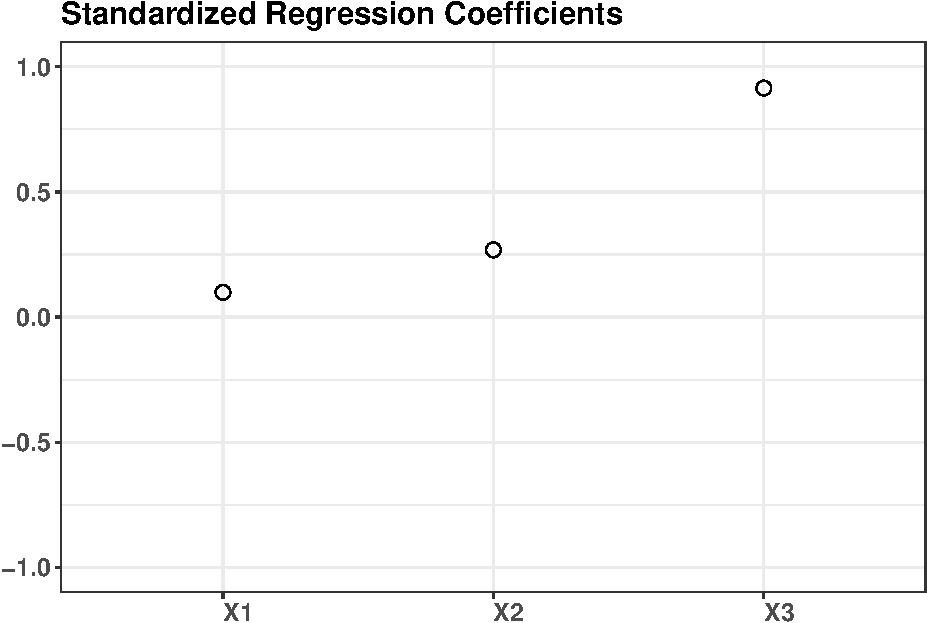
\includegraphics{topics_in_data_science_files/figure-latex/unnamed-chunk-3-1.pdf}

\begin{Shaded}
\begin{Highlighting}[]
\NormalTok{y <-}\StringTok{ }\KeywordTok{with}\NormalTok{(X, X1 }\OperatorTok{+}\StringTok{ }\NormalTok{X2 }\OperatorTok{+}\StringTok{ }\NormalTok{X3)}
\NormalTok{y <-}\StringTok{ }\NormalTok{y }\OperatorTok{+}\StringTok{ }\KeywordTok{rnorm}\NormalTok{(}\KeywordTok{nrow}\NormalTok{(X),}\DecValTok{0}\NormalTok{,}\DecValTok{1}\OperatorTok{/}\DecValTok{2}\NormalTok{)}
\NormalTok{df<-}\StringTok{ }\KeywordTok{data.frame}\NormalTok{(}\KeywordTok{cbind}\NormalTok{(X,y))}

\NormalTok{Z <-}\StringTok{ }\KeywordTok{src}\NormalTok{(X, y, }\DataTypeTok{rank =} \OtherTok{FALSE}\NormalTok{, }\DataTypeTok{logistic =} \OtherTok{FALSE}\NormalTok{, }\DataTypeTok{nboot =} \DecValTok{0}\NormalTok{, }\DataTypeTok{conf =} \FloatTok{0.95}\NormalTok{)}

\KeywordTok{pander}\NormalTok{(Z}\OperatorTok{$}\NormalTok{SRC,}\DataTypeTok{caption =} \StringTok{"Standardized Regression Coefficients "}\NormalTok{)}
\end{Highlighting}
\end{Shaded}

\begin{longtable}[]{@{}cc@{}}
\caption{Standardized Regression Coefficients}\tabularnewline
\toprule
\begin{minipage}[b]{0.12\columnwidth}\centering
~\strut
\end{minipage} & \begin{minipage}[b]{0.14\columnwidth}\centering
original\strut
\end{minipage}\tabularnewline
\midrule
\endfirsthead
\toprule
\begin{minipage}[b]{0.12\columnwidth}\centering
~\strut
\end{minipage} & \begin{minipage}[b]{0.14\columnwidth}\centering
original\strut
\end{minipage}\tabularnewline
\midrule
\endhead
\begin{minipage}[t]{0.12\columnwidth}\centering
\textbf{X1}\strut
\end{minipage} & \begin{minipage}[t]{0.14\columnwidth}\centering
0.1197\strut
\end{minipage}\tabularnewline
\begin{minipage}[t]{0.12\columnwidth}\centering
\textbf{X2}\strut
\end{minipage} & \begin{minipage}[t]{0.14\columnwidth}\centering
0.2438\strut
\end{minipage}\tabularnewline
\begin{minipage}[t]{0.12\columnwidth}\centering
\textbf{X3}\strut
\end{minipage} & \begin{minipage}[t]{0.14\columnwidth}\centering
0.906\strut
\end{minipage}\tabularnewline
\bottomrule
\end{longtable}

\begin{Shaded}
\begin{Highlighting}[]
\KeywordTok{ggplot}\NormalTok{(Z, }\DataTypeTok{ylim =} \KeywordTok{c}\NormalTok{(}\OperatorTok{-}\DecValTok{1}\NormalTok{,}\DecValTok{1}\NormalTok{))}\OperatorTok{+}\KeywordTok{ggtitle}\NormalTok{(}\StringTok{"Standardized Regression Coefficients"}\NormalTok{)}
\end{Highlighting}
\end{Shaded}

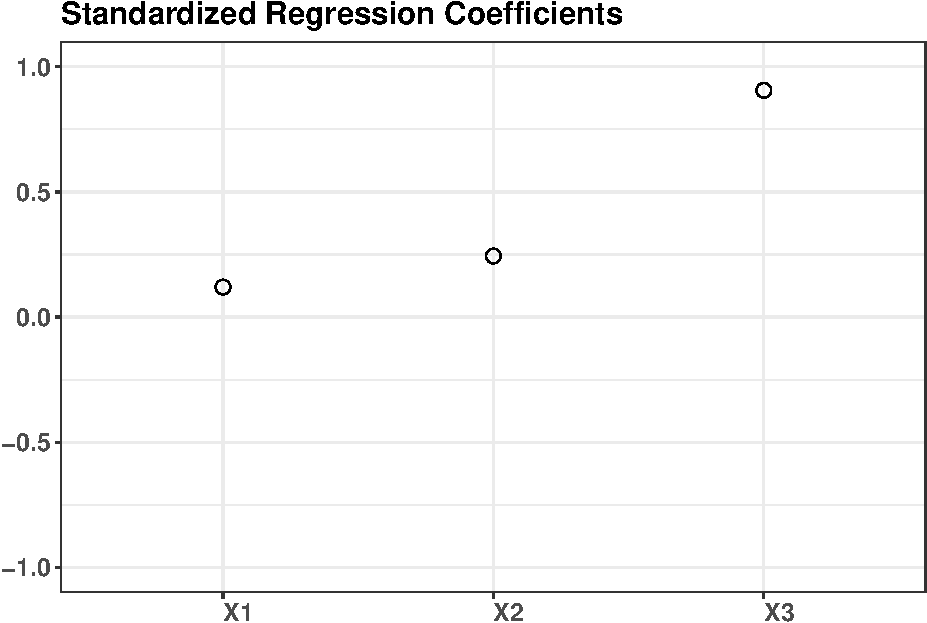
\includegraphics{topics_in_data_science_files/figure-latex/unnamed-chunk-4-1.pdf}

\begin{Shaded}
\begin{Highlighting}[]
\CommentTok{#lm.fit = lm(y ~ X1+X2+X3,data = df)}
\CommentTok{#summary(lm.fit)}
\CommentTok{#attach(df)}
\CommentTok{#plot(y, X1+X2+X3)}
\end{Highlighting}
\end{Shaded}

We see how the importance of X3 is ranked above X2 and likewise X2 is more important than X1. This is by design of the simulated data set. The standardized regression coefficients (beta coefficients) are calculated from that has been standardized, let's normalize and calculate the regression to see if indeed that is the case.

\begin{Shaded}
\begin{Highlighting}[]
\NormalTok{dfs<-}\StringTok{ }\KeywordTok{data.frame}\NormalTok{(}\KeywordTok{scale}\NormalTok{(df,}\DataTypeTok{center =} \OtherTok{TRUE}\NormalTok{,}\DataTypeTok{scale =} \OtherTok{TRUE}\NormalTok{))}
\NormalTok{lm.fit =}\StringTok{ }\KeywordTok{lm}\NormalTok{(y }\OperatorTok{~}\StringTok{ }\NormalTok{X1}\OperatorTok{+}\NormalTok{X2}\OperatorTok{+}\NormalTok{X3,}\DataTypeTok{data =}\NormalTok{ dfs)}
\KeywordTok{summary}\NormalTok{(lm.fit)}
\end{Highlighting}
\end{Shaded}

\begin{verbatim}
## 
## Call:
## lm(formula = y ~ X1 + X2 + X3, data = dfs)
## 
## Residuals:
##      Min       1Q   Median       3Q      Max 
## -0.46115 -0.09830 -0.01159  0.09760  0.36208 
## 
## Coefficients:
##               Estimate Std. Error t value Pr(>|t|)    
## (Intercept) -4.074e-16  1.709e-02   0.000        1    
## X1           1.197e-01  1.728e-02   6.926 4.92e-10 ***
## X2           2.438e-01  1.739e-02  14.017  < 2e-16 ***
## X3           9.060e-01  1.734e-02  52.237  < 2e-16 ***
## ---
## Signif. codes:  0 '***' 0.001 '**' 0.01 '*' 0.05 '.' 0.1 ' ' 1
## 
## Residual standard error: 0.1709 on 96 degrees of freedom
## Multiple R-squared:  0.9717, Adjusted R-squared:  0.9708 
## F-statistic:  1098 on 3 and 96 DF,  p-value: < 2.2e-16
\end{verbatim}

We see that the values are very close.

\hypertarget{partial-correlation-coefficients}{%
\section{Partial Correlation Coefficients}\label{partial-correlation-coefficients}}

\begin{Shaded}
\begin{Highlighting}[]
\NormalTok{x <-}\StringTok{ }\KeywordTok{pcc}\NormalTok{(X, y, }\DataTypeTok{nboot =} \DecValTok{100}\NormalTok{)}
\KeywordTok{print}\NormalTok{(x)}
\end{Highlighting}
\end{Shaded}

\begin{verbatim}
## 
## Call:
## pcc(X = X, y = y, nboot = 100)
## 
## Partial Correlation Coefficients (PCC):
##     original         bias  std. error min. c.i. max. c.i.
## X1 0.5772293 0.0056380312 0.067064354 0.4471891 0.7179550
## X2 0.8196099 0.0025391757 0.029985334 0.7653207 0.8848415
## X3 0.9828602 0.0005686946 0.002284419 0.9779532 0.9884970
\end{verbatim}

\hypertarget{sobol-indices-for-deterministic-function-and-for-model}{%
\section{Sobol indices for deterministic function and for model}\label{sobol-indices-for-deterministic-function-and-for-model}}

\begin{Shaded}
\begin{Highlighting}[]
\NormalTok{y.fun <-}\StringTok{ }\ControlFlowTok{function}\NormalTok{(X) \{}
  
\NormalTok{  X1<-}\StringTok{ }\NormalTok{X[,}\DecValTok{1}\NormalTok{]}
\NormalTok{  X2<-}\StringTok{ }\NormalTok{X[,}\DecValTok{2}\NormalTok{]}
\NormalTok{  X3<-}\StringTok{ }\NormalTok{X[,}\DecValTok{3}\NormalTok{]}
  
\NormalTok{  X1}\OperatorTok{+}\NormalTok{X2}\OperatorTok{+}\NormalTok{X3}
\NormalTok{\}}

\NormalTok{yhat.fun<-}\ControlFlowTok{function}\NormalTok{(X,lm)}
\NormalTok{\{}
\NormalTok{  X1<-}\StringTok{ }\NormalTok{X[,}\DecValTok{1}\NormalTok{]}
\NormalTok{  X2<-}\StringTok{ }\NormalTok{X[,}\DecValTok{2}\NormalTok{]}
\NormalTok{  X3<-}\StringTok{ }\NormalTok{X[,}\DecValTok{3}\NormalTok{]}
  
\NormalTok{  yhat <-}\StringTok{ }\KeywordTok{predict}\NormalTok{(lm.fit,}\KeywordTok{data.frame}\NormalTok{(}\DataTypeTok{X1=}\NormalTok{X1,}\DataTypeTok{X2=}\NormalTok{X2,}\DataTypeTok{X3=}\NormalTok{X3))}
  \KeywordTok{return}\NormalTok{(yhat)}
\NormalTok{\}}

\NormalTok{nboot =}\StringTok{ }\DecValTok{1000}

\NormalTok{x <-}\StringTok{ }\KeywordTok{sobol}\NormalTok{(}\DataTypeTok{model =}\NormalTok{ y.fun, X[}\DecValTok{1}\OperatorTok{:}\DecValTok{50}\NormalTok{,], X[}\DecValTok{51}\OperatorTok{:}\DecValTok{100}\NormalTok{,], }\DataTypeTok{order =} \DecValTok{3}\NormalTok{, }\DataTypeTok{nboot =}\NormalTok{ nboot)}
\NormalTok{S.sobol <-}\StringTok{ }\NormalTok{x}\OperatorTok{$}\NormalTok{S}
\KeywordTok{pander}\NormalTok{(S.sobol)}
\end{Highlighting}
\end{Shaded}

\begin{longtable}[]{@{}cccccc@{}}
\toprule
\begin{minipage}[b]{0.17\columnwidth}\centering
~\strut
\end{minipage} & \begin{minipage}[b]{0.12\columnwidth}\centering
original\strut
\end{minipage} & \begin{minipage}[b]{0.13\columnwidth}\centering
bias\strut
\end{minipage} & \begin{minipage}[b]{0.14\columnwidth}\centering
std. error\strut
\end{minipage} & \begin{minipage}[b]{0.13\columnwidth}\centering
min. c.i.\strut
\end{minipage} & \begin{minipage}[b]{0.13\columnwidth}\centering
max. c.i.\strut
\end{minipage}\tabularnewline
\midrule
\endhead
\begin{minipage}[t]{0.17\columnwidth}\centering
\textbf{X1}\strut
\end{minipage} & \begin{minipage}[t]{0.12\columnwidth}\centering
0.3045\strut
\end{minipage} & \begin{minipage}[t]{0.13\columnwidth}\centering
0.01067\strut
\end{minipage} & \begin{minipage}[t]{0.14\columnwidth}\centering
0.8787\strut
\end{minipage} & \begin{minipage}[t]{0.13\columnwidth}\centering
-1.464\strut
\end{minipage} & \begin{minipage}[t]{0.13\columnwidth}\centering
1.949\strut
\end{minipage}\tabularnewline
\begin{minipage}[t]{0.17\columnwidth}\centering
\textbf{X2}\strut
\end{minipage} & \begin{minipage}[t]{0.12\columnwidth}\centering
0.1629\strut
\end{minipage} & \begin{minipage}[t]{0.13\columnwidth}\centering
-0.003125\strut
\end{minipage} & \begin{minipage}[t]{0.14\columnwidth}\centering
0.8411\strut
\end{minipage} & \begin{minipage}[t]{0.13\columnwidth}\centering
-1.43\strut
\end{minipage} & \begin{minipage}[t]{0.13\columnwidth}\centering
1.754\strut
\end{minipage}\tabularnewline
\begin{minipage}[t]{0.17\columnwidth}\centering
\textbf{X3}\strut
\end{minipage} & \begin{minipage}[t]{0.12\columnwidth}\centering
1.485\strut
\end{minipage} & \begin{minipage}[t]{0.13\columnwidth}\centering
0.0379\strut
\end{minipage} & \begin{minipage}[t]{0.14\columnwidth}\centering
0.2252\strut
\end{minipage} & \begin{minipage}[t]{0.13\columnwidth}\centering
0.9809\strut
\end{minipage} & \begin{minipage}[t]{0.13\columnwidth}\centering
1.873\strut
\end{minipage}\tabularnewline
\begin{minipage}[t]{0.17\columnwidth}\centering
**X1*X2**\strut
\end{minipage} & \begin{minipage}[t]{0.12\columnwidth}\centering
-0.3074\strut
\end{minipage} & \begin{minipage}[t]{0.13\columnwidth}\centering
-0.01577\strut
\end{minipage} & \begin{minipage}[t]{0.14\columnwidth}\centering
0.8972\strut
\end{minipage} & \begin{minipage}[t]{0.13\columnwidth}\centering
-1.956\strut
\end{minipage} & \begin{minipage}[t]{0.13\columnwidth}\centering
1.464\strut
\end{minipage}\tabularnewline
\begin{minipage}[t]{0.17\columnwidth}\centering
**X1*X3**\strut
\end{minipage} & \begin{minipage}[t]{0.12\columnwidth}\centering
-0.3074\strut
\end{minipage} & \begin{minipage}[t]{0.13\columnwidth}\centering
-0.01577\strut
\end{minipage} & \begin{minipage}[t]{0.14\columnwidth}\centering
0.8972\strut
\end{minipage} & \begin{minipage}[t]{0.13\columnwidth}\centering
-1.956\strut
\end{minipage} & \begin{minipage}[t]{0.13\columnwidth}\centering
1.464\strut
\end{minipage}\tabularnewline
\begin{minipage}[t]{0.17\columnwidth}\centering
**X2*X3**\strut
\end{minipage} & \begin{minipage}[t]{0.12\columnwidth}\centering
-0.3074\strut
\end{minipage} & \begin{minipage}[t]{0.13\columnwidth}\centering
-0.01577\strut
\end{minipage} & \begin{minipage}[t]{0.14\columnwidth}\centering
0.8972\strut
\end{minipage} & \begin{minipage}[t]{0.13\columnwidth}\centering
-1.956\strut
\end{minipage} & \begin{minipage}[t]{0.13\columnwidth}\centering
1.464\strut
\end{minipage}\tabularnewline
\begin{minipage}[t]{0.17\columnwidth}\centering
\textbf{X1\emph{X2}X3}\strut
\end{minipage} & \begin{minipage}[t]{0.12\columnwidth}\centering
0.3074\strut
\end{minipage} & \begin{minipage}[t]{0.13\columnwidth}\centering
0.01577\strut
\end{minipage} & \begin{minipage}[t]{0.14\columnwidth}\centering
0.8972\strut
\end{minipage} & \begin{minipage}[t]{0.13\columnwidth}\centering
-1.464\strut
\end{minipage} & \begin{minipage}[t]{0.13\columnwidth}\centering
1.956\strut
\end{minipage}\tabularnewline
\bottomrule
\end{longtable}

\begin{Shaded}
\begin{Highlighting}[]
\CommentTok{#yhat.fun(data.frame(X1=1,X2=2,X3=3),lm.fit)}

\NormalTok{x <-}\StringTok{ }\KeywordTok{sobol}\NormalTok{(}\DataTypeTok{model =}\NormalTok{ yhat.fun,X[}\DecValTok{1}\OperatorTok{:}\DecValTok{50}\NormalTok{,], X[}\DecValTok{51}\OperatorTok{:}\DecValTok{100}\NormalTok{,], }\DataTypeTok{order =} \DecValTok{3}\NormalTok{, }\DataTypeTok{nboot =}\NormalTok{ nboot)}
\NormalTok{S.sobol <-}\StringTok{ }\NormalTok{x}\OperatorTok{$}\NormalTok{S}
\KeywordTok{pander}\NormalTok{(S.sobol)}
\end{Highlighting}
\end{Shaded}

\begin{longtable}[]{@{}cccccc@{}}
\toprule
\begin{minipage}[b]{0.17\columnwidth}\centering
~\strut
\end{minipage} & \begin{minipage}[b]{0.13\columnwidth}\centering
original\strut
\end{minipage} & \begin{minipage}[b]{0.12\columnwidth}\centering
bias\strut
\end{minipage} & \begin{minipage}[b]{0.14\columnwidth}\centering
std. error\strut
\end{minipage} & \begin{minipage}[b]{0.13\columnwidth}\centering
min. c.i.\strut
\end{minipage} & \begin{minipage}[b]{0.13\columnwidth}\centering
max. c.i.\strut
\end{minipage}\tabularnewline
\midrule
\endhead
\begin{minipage}[t]{0.17\columnwidth}\centering
\textbf{X1}\strut
\end{minipage} & \begin{minipage}[t]{0.13\columnwidth}\centering
7.339e-05\strut
\end{minipage} & \begin{minipage}[t]{0.12\columnwidth}\centering
-0.04067\strut
\end{minipage} & \begin{minipage}[t]{0.14\columnwidth}\centering
0.7359\strut
\end{minipage} & \begin{minipage}[t]{0.13\columnwidth}\centering
-1.386\strut
\end{minipage} & \begin{minipage}[t]{0.13\columnwidth}\centering
1.419\strut
\end{minipage}\tabularnewline
\begin{minipage}[t]{0.17\columnwidth}\centering
\textbf{X2}\strut
\end{minipage} & \begin{minipage}[t]{0.13\columnwidth}\centering
-0.03858\strut
\end{minipage} & \begin{minipage}[t]{0.12\columnwidth}\centering
-0.04091\strut
\end{minipage} & \begin{minipage}[t]{0.14\columnwidth}\centering
0.7296\strut
\end{minipage} & \begin{minipage}[t]{0.13\columnwidth}\centering
-1.393\strut
\end{minipage} & \begin{minipage}[t]{0.13\columnwidth}\centering
1.361\strut
\end{minipage}\tabularnewline
\begin{minipage}[t]{0.17\columnwidth}\centering
\textbf{X3}\strut
\end{minipage} & \begin{minipage}[t]{0.13\columnwidth}\centering
1.283\strut
\end{minipage} & \begin{minipage}[t]{0.12\columnwidth}\centering
0.01002\strut
\end{minipage} & \begin{minipage}[t]{0.14\columnwidth}\centering
0.0622\strut
\end{minipage} & \begin{minipage}[t]{0.13\columnwidth}\centering
1.136\strut
\end{minipage} & \begin{minipage}[t]{0.13\columnwidth}\centering
1.385\strut
\end{minipage}\tabularnewline
\begin{minipage}[t]{0.17\columnwidth}\centering
**X1*X2**\strut
\end{minipage} & \begin{minipage}[t]{0.13\columnwidth}\centering
-0.001133\strut
\end{minipage} & \begin{minipage}[t]{0.12\columnwidth}\centering
0.04042\strut
\end{minipage} & \begin{minipage}[t]{0.14\columnwidth}\centering
0.738\strut
\end{minipage} & \begin{minipage}[t]{0.13\columnwidth}\centering
-1.408\strut
\end{minipage} & \begin{minipage}[t]{0.13\columnwidth}\centering
1.396\strut
\end{minipage}\tabularnewline
\begin{minipage}[t]{0.17\columnwidth}\centering
**X1*X3**\strut
\end{minipage} & \begin{minipage}[t]{0.13\columnwidth}\centering
-0.001133\strut
\end{minipage} & \begin{minipage}[t]{0.12\columnwidth}\centering
0.04042\strut
\end{minipage} & \begin{minipage}[t]{0.14\columnwidth}\centering
0.738\strut
\end{minipage} & \begin{minipage}[t]{0.13\columnwidth}\centering
-1.408\strut
\end{minipage} & \begin{minipage}[t]{0.13\columnwidth}\centering
1.396\strut
\end{minipage}\tabularnewline
\begin{minipage}[t]{0.17\columnwidth}\centering
**X2*X3**\strut
\end{minipage} & \begin{minipage}[t]{0.13\columnwidth}\centering
-0.001133\strut
\end{minipage} & \begin{minipage}[t]{0.12\columnwidth}\centering
0.04042\strut
\end{minipage} & \begin{minipage}[t]{0.14\columnwidth}\centering
0.738\strut
\end{minipage} & \begin{minipage}[t]{0.13\columnwidth}\centering
-1.408\strut
\end{minipage} & \begin{minipage}[t]{0.13\columnwidth}\centering
1.396\strut
\end{minipage}\tabularnewline
\begin{minipage}[t]{0.17\columnwidth}\centering
\textbf{X1\emph{X2}X3}\strut
\end{minipage} & \begin{minipage}[t]{0.13\columnwidth}\centering
0.001133\strut
\end{minipage} & \begin{minipage}[t]{0.12\columnwidth}\centering
-0.04042\strut
\end{minipage} & \begin{minipage}[t]{0.14\columnwidth}\centering
0.738\strut
\end{minipage} & \begin{minipage}[t]{0.13\columnwidth}\centering
-1.396\strut
\end{minipage} & \begin{minipage}[t]{0.13\columnwidth}\centering
1.408\strut
\end{minipage}\tabularnewline
\bottomrule
\end{longtable}

\hypertarget{on-model-averaging}{%
\chapter{On Model Averaging}\label{on-model-averaging}}

Recall that we can break down model error into the bias an variance \(bias(\hat{Y})= E[\hat{Y}-E[Y]]\)

If we are averaging models \(i=1, \cdots ,k\) then

\(\operatorname{MSE}\left(\hat{Y}_{i}\right)=\left\{\operatorname{bias}\left(\hat{Y}_{i}\right)\right\}^{2}+\operatorname{var}\left(\hat{Y}_{i}\right)\)

\hypertarget{poincare-embedding}{%
\chapter{Poincare Embedding}\label{poincare-embedding}}

\hypertarget{embeddings}{%
\section{Embeddings}\label{embeddings}}

\emph{The Poincaré Embedding is concerned with the problem of learning hierarchical structure on the dataset. Phylogenetic tree or the tree of hypernymy are the examples of hierarchical structure dataset. The embedding space is a Poincaré ball, which is an unit ball equipped with poincaré distance. An advantage using Poincaré space compared to the Euclidean space as embedding space is that this space preserve tree-shaped structure well in relatively low dimension. This is because poincaré distance is intuitively continuous version of distance on tree-shaped dataset. We can take advantage of this property to provide efficient embeddings with comparably less dimensionality.}

See {[}\url{https://github.com/hwchang1201/poincare.embeddings/}{]}

\citep{DBLP:journals/corr/NickelK17}

\citep{DBLP:journals/corr/abs-1806-03417}

\begin{Shaded}
\begin{Highlighting}[]
\KeywordTok{install.packages}\NormalTok{(}\StringTok{"remotes"}\NormalTok{)}
\end{Highlighting}
\end{Shaded}

\begin{verbatim}
## Installing package into '/home/bruce/R/x86_64-pc-linux-gnu-library/4.1'
## (as 'lib' is unspecified)
\end{verbatim}

\begin{Shaded}
\begin{Highlighting}[]
\NormalTok{remotes}\OperatorTok{::}\KeywordTok{install_github}\NormalTok{(}\StringTok{"hwchang1201/poincare.embeddings"}\NormalTok{, }\DataTypeTok{upgrade =} \StringTok{"never"}\NormalTok{)}
\end{Highlighting}
\end{Shaded}

\begin{verbatim}
## Skipping install of 'poincare.embeddings' from a github remote, the SHA1 (7fd455e0) has not changed since last install.
##   Use `force = TRUE` to force installation
\end{verbatim}

\begin{Shaded}
\begin{Highlighting}[]
\KeywordTok{install.packages}\NormalTok{(}\StringTok{'data.tree'}\NormalTok{)}
\end{Highlighting}
\end{Shaded}

\begin{verbatim}
## Installing package into '/home/bruce/R/x86_64-pc-linux-gnu-library/4.1'
## (as 'lib' is unspecified)
\end{verbatim}

\begin{Shaded}
\begin{Highlighting}[]
\KeywordTok{library}\NormalTok{(yaml)}
\KeywordTok{library}\NormalTok{(data.tree)}
\CommentTok{# defining tree structured dataset.}
\NormalTok{acme_treeDataset <-}\StringTok{ }\NormalTok{Node}\OperatorTok{$}\KeywordTok{new}\NormalTok{(}\StringTok{"Acme Inc."}\NormalTok{)}
\NormalTok{  accounting <-}\StringTok{ }\NormalTok{acme_treeDataset}\OperatorTok{$}\KeywordTok{AddChild}\NormalTok{(}\StringTok{"Accounting"}\NormalTok{)}
\NormalTok{    software <-}\StringTok{ }\NormalTok{accounting}\OperatorTok{$}\KeywordTok{AddChild}\NormalTok{(}\StringTok{"New Software"}\NormalTok{)}
\NormalTok{    standards <-}\StringTok{ }\NormalTok{accounting}\OperatorTok{$}\KeywordTok{AddChild}\NormalTok{(}\StringTok{"New Accounting Standards"}\NormalTok{)}
\NormalTok{  research <-}\StringTok{ }\NormalTok{acme_treeDataset}\OperatorTok{$}\KeywordTok{AddChild}\NormalTok{(}\StringTok{"Research"}\NormalTok{)}
\NormalTok{    newProductLine <-}\StringTok{ }\NormalTok{research}\OperatorTok{$}\KeywordTok{AddChild}\NormalTok{(}\StringTok{"New Product Line"}\NormalTok{)}
\NormalTok{    newLabs <-}\StringTok{ }\NormalTok{research}\OperatorTok{$}\KeywordTok{AddChild}\NormalTok{(}\StringTok{"New Labs"}\NormalTok{)}
\NormalTok{  it <-}\StringTok{ }\NormalTok{acme_treeDataset}\OperatorTok{$}\KeywordTok{AddChild}\NormalTok{(}\StringTok{"IT"}\NormalTok{)}
\NormalTok{    outsource <-}\StringTok{ }\NormalTok{it}\OperatorTok{$}\KeywordTok{AddChild}\NormalTok{(}\StringTok{"Outsource"}\NormalTok{)}
\NormalTok{    agile <-}\StringTok{ }\NormalTok{it}\OperatorTok{$}\KeywordTok{AddChild}\NormalTok{(}\StringTok{"Go agile"}\NormalTok{)}
\NormalTok{    goToR <-}\StringTok{ }\NormalTok{it}\OperatorTok{$}\KeywordTok{AddChild}\NormalTok{(}\StringTok{"Switch to R"}\NormalTok{)}

\KeywordTok{print}\NormalTok{(acme_treeDataset)}
\end{Highlighting}
\end{Shaded}

\begin{verbatim}
##                           levelName
## 1  Acme Inc.                       
## 2   ¦--Accounting                  
## 3   ¦   ¦--New Software            
## 4   ¦   °--New Accounting Standards
## 5   ¦--Research                    
## 6   ¦   ¦--New Product Line        
## 7   ¦   °--New Labs                
## 8   °--IT                          
## 9       ¦--Outsource               
## 10      ¦--Go agile                
## 11      °--Switch to R
\end{verbatim}

\begin{Shaded}
\begin{Highlighting}[]
\CommentTok{# loading package "poincare.embeddings"}
\KeywordTok{library}\NormalTok{(poincare.embeddings)}

\CommentTok{# use example dataset}
\CommentTok{# 1. use "toy"}
\NormalTok{toy_yaml <-}\StringTok{ }\NormalTok{yaml}\OperatorTok{::}\KeywordTok{yaml.load}\NormalTok{(toy)}
\NormalTok{toy_tree <-}\StringTok{ }\NormalTok{data.tree}\OperatorTok{::}\KeywordTok{as.Node}\NormalTok{(toy_yaml)}
\NormalTok{emb <-}\StringTok{ }\KeywordTok{poincareEmbeddings}\NormalTok{(toy_tree, }\DataTypeTok{theta_dim =} \DecValTok{2}\NormalTok{, }\DataTypeTok{N_epoch =} \DecValTok{200}\NormalTok{, }\DataTypeTok{lr =} \FloatTok{0.05}\NormalTok{, }\DataTypeTok{n_neg =} \DecValTok{10}\NormalTok{)}
\end{Highlighting}
\end{Shaded}

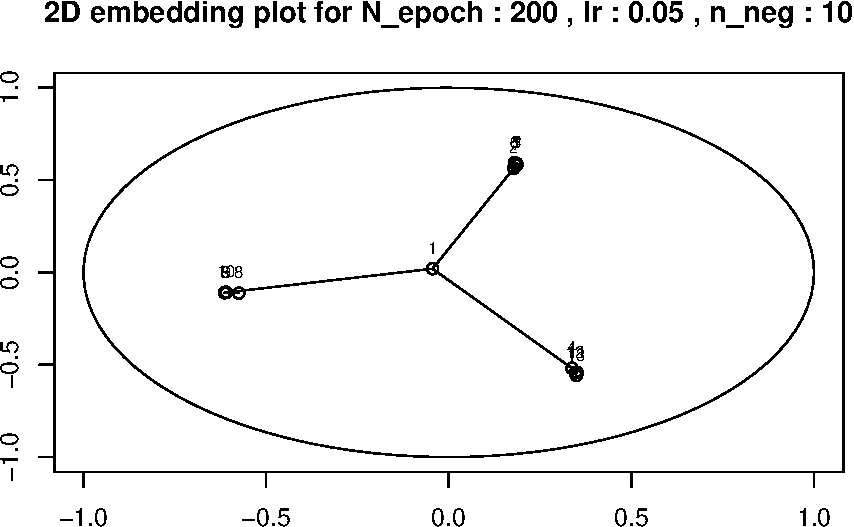
\includegraphics{topics_in_data_science_files/figure-latex/unnamed-chunk-9-1.pdf}

\begin{Shaded}
\begin{Highlighting}[]
\CommentTok{# 2. use "statistics"}
\NormalTok{statistics_yaml <-}\StringTok{ }\NormalTok{yaml}\OperatorTok{::}\KeywordTok{yaml.load}\NormalTok{(statistics)}
\NormalTok{statistics_tree <-}\StringTok{ }\NormalTok{data.tree}\OperatorTok{::}\KeywordTok{as.Node}\NormalTok{(statistics_yaml)}
\NormalTok{emb <-}\StringTok{ }\KeywordTok{poincareEmbeddings}\NormalTok{(statistics_tree, }\DataTypeTok{theta_dim =} \DecValTok{2}\NormalTok{, }\DataTypeTok{N_epoch =} \DecValTok{200}\NormalTok{, }\DataTypeTok{lr =} \FloatTok{0.05}\NormalTok{, }\DataTypeTok{n_neg =} \DecValTok{10}\NormalTok{)}
\end{Highlighting}
\end{Shaded}

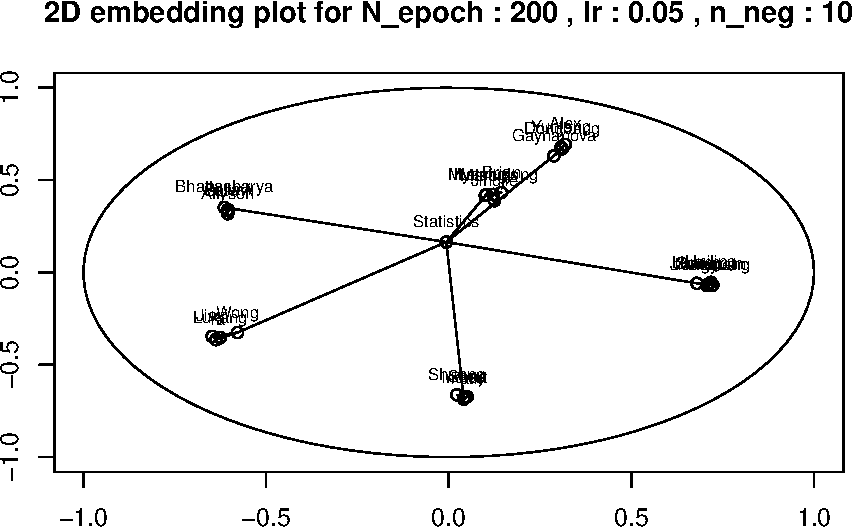
\includegraphics{topics_in_data_science_files/figure-latex/unnamed-chunk-9-2.pdf}

\begin{Shaded}
\begin{Highlighting}[]
\CommentTok{# 3. use "statistics_adv"}
\NormalTok{statistics_adv_yaml <-}\StringTok{ }\NormalTok{yaml}\OperatorTok{::}\KeywordTok{yaml.load}\NormalTok{(statistics_adv)}
\NormalTok{statistics_adv_tree <-}\StringTok{ }\NormalTok{data.tree}\OperatorTok{::}\KeywordTok{as.Node}\NormalTok{(statistics_adv_yaml)}
\NormalTok{emb <-}\StringTok{ }\KeywordTok{poincareEmbeddings}\NormalTok{(statistics_adv_tree, }\DataTypeTok{theta_dim =} \DecValTok{2}\NormalTok{, }\DataTypeTok{N_epoch =} \DecValTok{200}\NormalTok{, }\DataTypeTok{lr =} \FloatTok{0.05}\NormalTok{, }\DataTypeTok{n_neg =} \DecValTok{10}\NormalTok{)}
\end{Highlighting}
\end{Shaded}

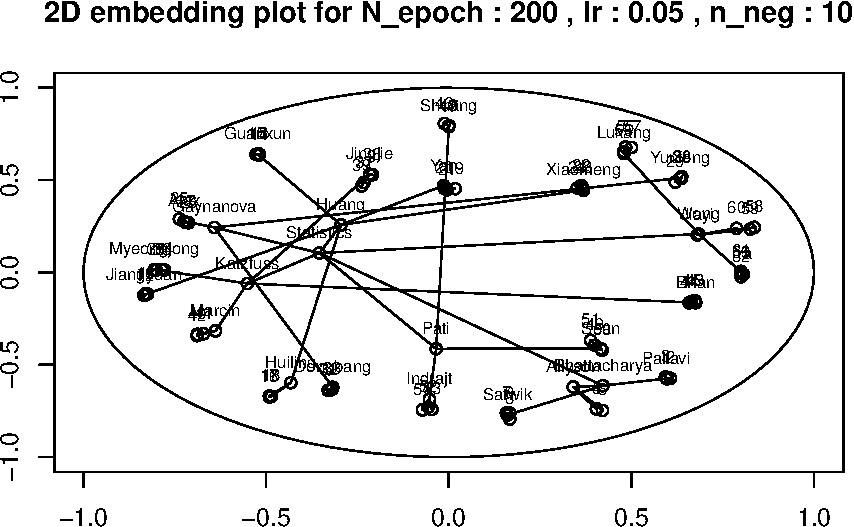
\includegraphics{topics_in_data_science_files/figure-latex/unnamed-chunk-9-3.pdf}

\begin{Shaded}
\begin{Highlighting}[]
\KeywordTok{print}\NormalTok{(}\KeywordTok{paste}\NormalTok{(}\StringTok{"The ranking of the poincare embedding :"}\NormalTok{, emb}\OperatorTok{$}\NormalTok{rank))}
\end{Highlighting}
\end{Shaded}

\begin{verbatim}
## [1] "The ranking of the poincare embedding : 5.48888888888889"
\end{verbatim}

\begin{Shaded}
\begin{Highlighting}[]
\KeywordTok{print}\NormalTok{(}\KeywordTok{paste}\NormalTok{(}\StringTok{"The mean average precision of the poincare embedding :"}\NormalTok{, emb}\OperatorTok{$}\NormalTok{map))}
\end{Highlighting}
\end{Shaded}

\begin{verbatim}
## [1] "The mean average precision of the poincare embedding : 0.73738246401919"
\end{verbatim}

\hypertarget{multirelational}{%
\chapter{Multirelational}\label{multirelational}}

\url{https://github.com/ibalazevic/multirelational-poincare}

GeomStats
\url{https://geomstats.github.io/geomstats.github.io/05_embedding_graph_structured_data_h2.html}

\hypertarget{mlops}{%
\chapter{MLOps}\label{mlops}}

\emph{Development platform: a collaborative platform for performing ML experiments and empowering the creation of ML models by data scientists should be considered part of the MLOps framework. This platform should enable secure access to data sources (e.g.~from data engineering workflows). We want the handover from ML training to deployment to be as smooth as possible, which is more likely the case for such a platform as compared to ML models developed in different local environment.
Model unit testing: every time we create, change, or retrain a model, we should automatically validate the integrity of the model, e.g.
- should meet minimum performance on test set
- should perform well on synthetic use case-specific datasets
Versioning: it should be possible to go back in time to inspect everything relating to a given model; e.g.~what data \& code was used. Why? because it something breaks, we need to be able to go back in time and see why.
Model registry: there should be an overview of deployed \& decommissioned ML models, their version history, and deployment stage of each version. Why? if something breaks, we can rollback a previous archived version back into production.
Model Governance: only certain people should have access to see training related to any given model, and there should be access control for who can request/reject/approve transitions between deployment stages (e.g.~dev to test to prod) in the model registry.
Deployments: deployment can be many things, but in this post I consider the case where we want to deploy a model to cloud infrastructure and expose an API, which enables other people to consume and use the model, i.e.~I'm not considering cases where we want to deploy ML models into embedded systems. Efficient model deployments on appropriate infrastructure should:
- support multiple ML frameworks + custom models
- have well defined API spec (e.g.~Swagger/OpenAPI)
- support containerized model servers
Monitoring: tracking performance metrics (throughput, uptime, etc.). Why? If all of the sudden a model starts returning errors, or being unexpectedly slow, we need to know before the end-user complains, so that we can fix it.
Feedback: we need to feedback information to the model on how well it is performing. Why? typically we run predictions on new samples where we do not yet know the ground truth. As we learn the truth, however, we need to inform the model, so that it can report on how well it is actually doing.
A/B testing: no matter how solid cross-validation we think we're doing, we never know how the model will perform until it actually gets deployed. It should be easy to perform A/B experiments with live models within the MLOps framework.
Drift detection: typically the longer time a given model is deployed the worse it becomes as circumstances change compared to the time of training the model. We can try to monitor and alert on these different circumstances, or ``drifts'', before they get too severe:
- Concept drift: when the relation between input and output has changed
- Prediction drift: changes in incoming predictions, but model still holds
- Label drift: change in the model's outcomes compared to training data
- Feature drift: change in the distribution of model input data
Outlier detection: if a deployed model receives an input sample which is significantly different from anything observed during training, we can try to identify this sample as a potential outlier, and the returned prediction should be marked as such, indicating that the end-user should be careful in trusting the prediction.
Adversarial Attack Detection: we should be warned when our models are attacked by adversarial samples (e.g.~someone trying to abuse / manipulate the outcome of our algorithms).
Interpretability: the ML deployments should support endpoints returning the explanation of our prediction, e.g.~through SHAP values. Why? for a lot of use cases a prediction is not enough and the end-user needs to know why a given prediction was made.
Governance of deployments: we not only need access restrictions on who can see the data, trained models, etc, but also for who can eventually use the deployed models. These deployed models can often be just as confidential as the data they were trained on.
Data-centricity: rather than focus on model performance \& improvements, it makes sense that a MLOps framework also enables an increased focus on how data quality and breadth can be improved.}

\hypertarget{introduction-to-normalizing-flows}{%
\chapter{Introduction to Normalizing Flows}\label{introduction-to-normalizing-flows}}

\hypertarget{variational-inference-with-nf}{%
\section{Variational Inference With NF}\label{variational-inference-with-nf}}

\emph{Variational inference now lies at the core of large-scale topic models of text (Hoffman et al., 2013), provides the state-of-the-art in semi-supervised classification (Kingma et al., 2014), drives the models that currently produce the most realistic generative models of images (Gregor et al., 2014; Rezende et al., 2014), and are a default Proceedings of the 32 nd International Conference on Machine Learning, Lille, France, 2015. JMLR: W\&CP volume 37. Copyright 2015 by the author(s). tool for the understanding of many physical and chemical systems. Despite these successes and ongoing advances, there are a number of disadvantages of variational methods that limit their power and hamper their wider adoption as a default method for statistical inference. It is one of these limitations, the choice of posterior approximation, that we address in this paper}

{[}\url{http://proceedings.mlr.press/v37/rezende15.pdf}{]}

\emph{Generative modeling loosely refers to building a model of data, for instance p(image), that we can sample from. This is in contrast to discriminative modeling, such as regression or classification, which tries to estimate conditional distributions such as p(class \textbar{} image).}

See also

\url{https://blog.evjang.com/2018/01/nf1.html}

\url{https://deepgenerativemodels.github.io/notes/flow}

\hypertarget{sa-and-m-estimators}{%
\chapter{SA and M-estimators}\label{sa-and-m-estimators}}

R. Martin and C. Masreliez, ``Robust estimation via stochastic approximation,'' in IEEE Transactions on Information Theory, vol.~21, no. 3, pp.~263-271, May 1975, doi: 10.1109/TIT.1975.1055386.

\hypertarget{random-matrix-theory-and-machine-learning}{%
\chapter{Random Matrix Theory and Machine Learning}\label{random-matrix-theory-and-machine-learning}}

  \bibliography{packages.bib,book.bib}

\end{document}
